\documentclass{ximera}

\input{../../preamble.tex}

\author{Vic Ferdinand, Betsy McNeal, Jenny Sheldon}
%\license{Creative Commons Attribution-ShareAlike 4.0 International License}
%\acknowledgement{https://activecalculus.org/prelude/sec-changing-in-tandem.html}

%\outcome{Understand the relationship between position, velocity and acceleration.}
%\outcome{Discuss the meaning of antiderivatives of a position function.}

\begin{document}
\begin{exercise}
For each of the situations below, pick the graph that most reasonably
reflects the situation and the variables involved.

\begin{enumerate}
\item \label{graphicDetailsA} The daily high temperature recorded in Chicago from January to
  December: $\answer{C}$
%Will it accept little c?

 \begin{image}
     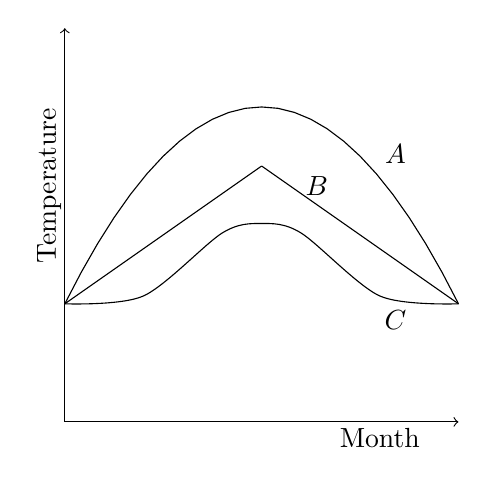
\begin{tikzpicture}
         \draw[->](0,0)--(5,0);
         \draw[->](0,0)--(0,5);
         \node at (4, -0.2) {Month};
         \node[rotate=90] at (-0.2, 3) {Temperature};
         \draw[domain=0:5] plot (\x, {-0.4*(\x-2.5)^2+4});
         \node at (4.2, 3.4) {$A$};
         \draw[domain=0:2.5] plot (\x, {1.5+0.7*\x});
         \draw[domain=2.5:5] plot (\x, {3.25-0.7*(\x-2.5)});
         \node at (4.2, 1.3) {$C$};
         \draw plot[smooth] coordinates {(0,1.5) (1, 1.6) (2, 2.4) (2.5,2.52) (3,2.4) (4,1.6) (5,1.5)};
         \node at (3.2, 3) {$B$};
     \end{tikzpicture}
 \end{image}



\item \label{graphicDetailsB} The number of gallons of milk you can buy with $\$5$ as the cost per gallon of
  milk increases: $\answer{B}$

\begin{image}
    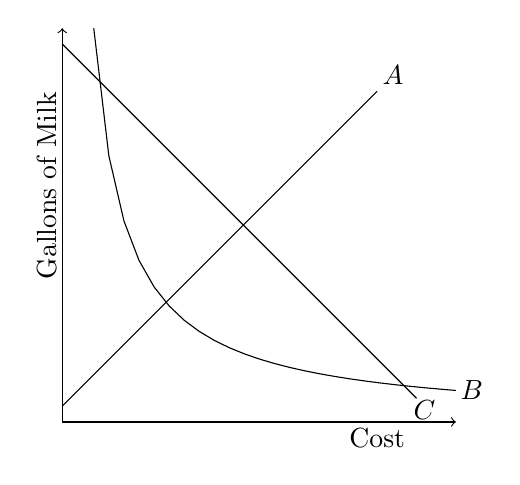
\begin{tikzpicture}
        \draw[->](0,0)--(5,0);
        \draw[->](0,0)--(0,5);
        \node at (4, -0.2) {Cost};
        \node[rotate=90] at (-0.2, 3) {Gallons of Milk};
        \draw[domain=0:4] plot (\x, {0.2+\x});
        \node at (4.2, 4.4) {$A$};
        \draw[domain=0:4.5] plot (\x, {4.8-\x});
        \node at (4.6, 0.15) {$C$};
        \draw[domain=0.4:5] plot (\x, {2/\x});
        \node at (5.2, 0.4) {$B$};
    \end{tikzpicture}
\end{image}

\end{enumerate}



%\begin{multipleChoice}
%\choice{constant function.}
%\choice{positive function. }
%\choice{negative function.}
%\choice{position function.}
%\choice[correct]{velocity function.}
%\end{multipleChoice}


\end{exercise}
\end{document}
